\section{Dual parachute design (Payload's Case)}\label{A4}
\coloredbox{CDOSRSecondary!50}{CDOSRPrimary}{CDOSRPrimary}{
    \begin{minipage}{0.4\textwidth}
    The smaller parachute had a diameter of 21.7 cm and a surface area of 370 cm$^{2}$, which is designed to slow down the descent speed to 9 meters per second. The design of this parachute was based on the principles of aerodynamics and is intended to withstand strong winds and turbulent weather conditions. We believe that this parachute will be instrumental in ensuring a safe and successful landing of our Payload during windy weather conditions.
    \end{minipage}
    \hfill
    \begin{minipage}{0.4\textwidth}
    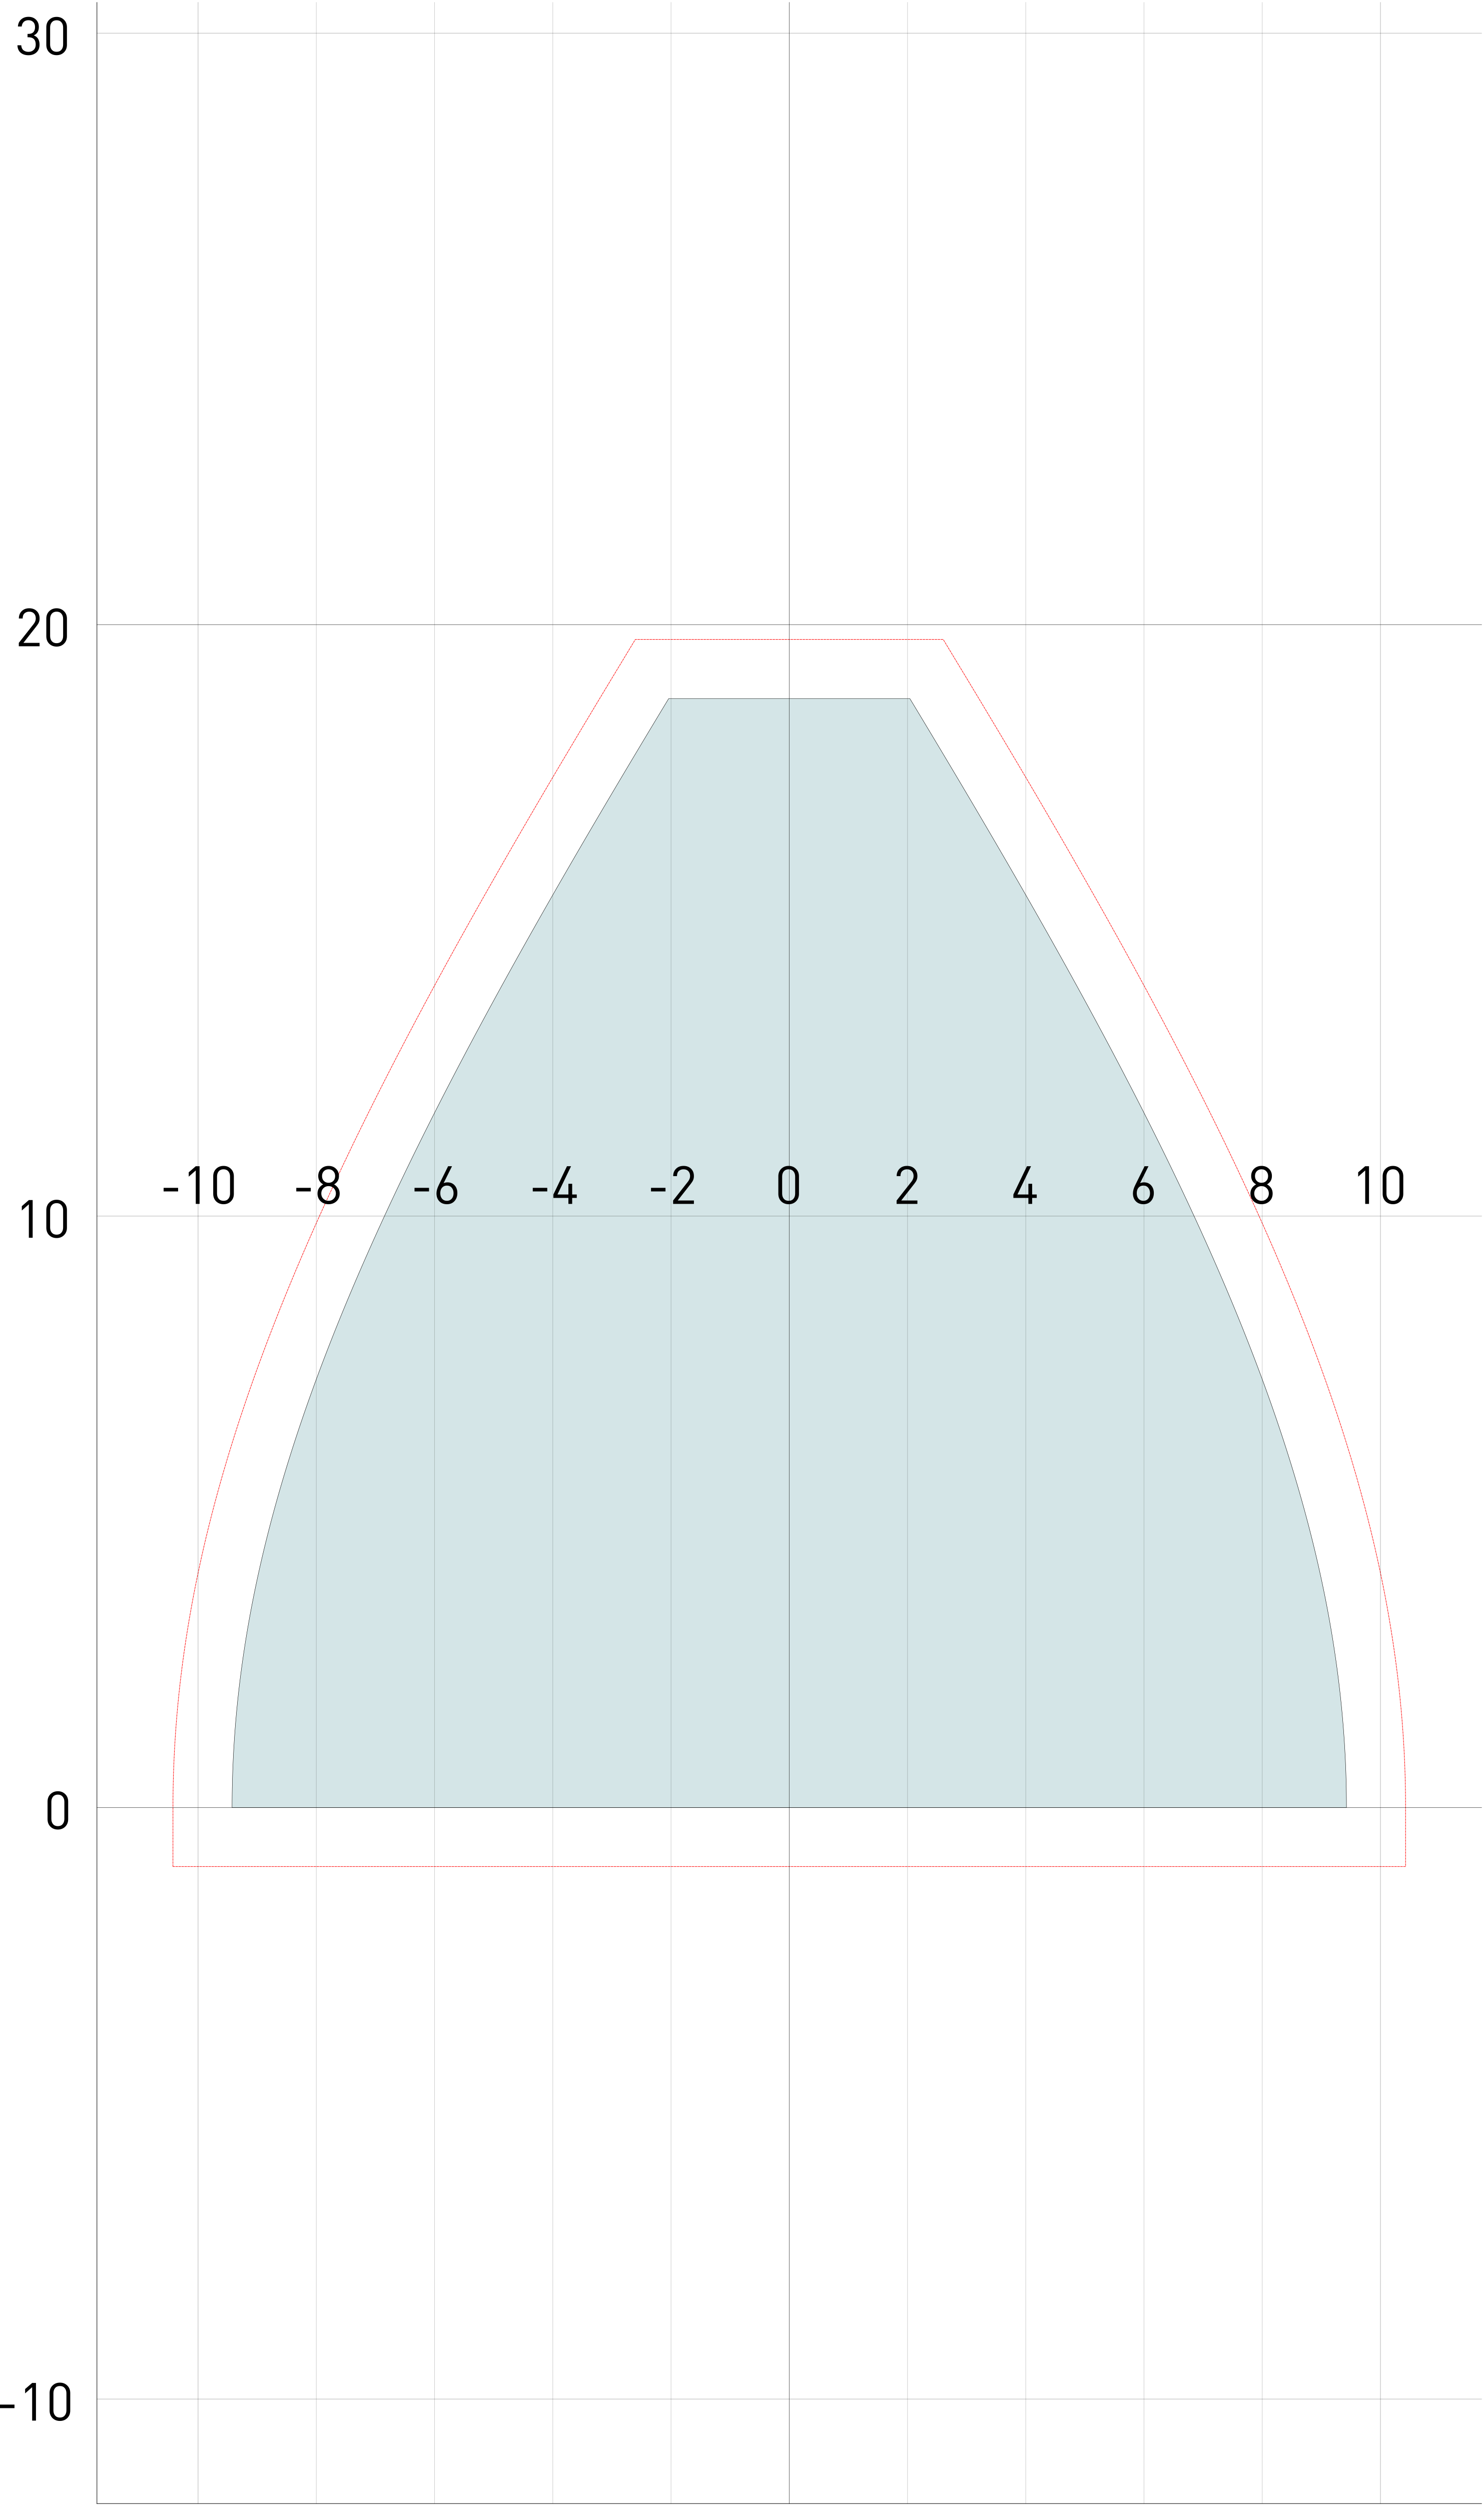
\includegraphics[width=5cm]{PlotItem_2.png}
    \end{minipage}
}
\coloredbox{CDOSRSecondary!50}{CDOSRPrimary}{CDOSRPrimary}{
    \begin{minipage}{0.4\textwidth}
    The second parachute was designed for use during calm weather conditions and had a diameter of 32.6 cm and a surface area of 834 cm$^{2}$, which is designed to slow down the descent speed to 6 meters per second. This parachute was optimized for stable and predictable conditions and is intended to provide a gentle and controlled descent of the Payload during calm weather conditions.
    \end{minipage}
    \hfill
    \begin{minipage}{0.4\textwidth}
    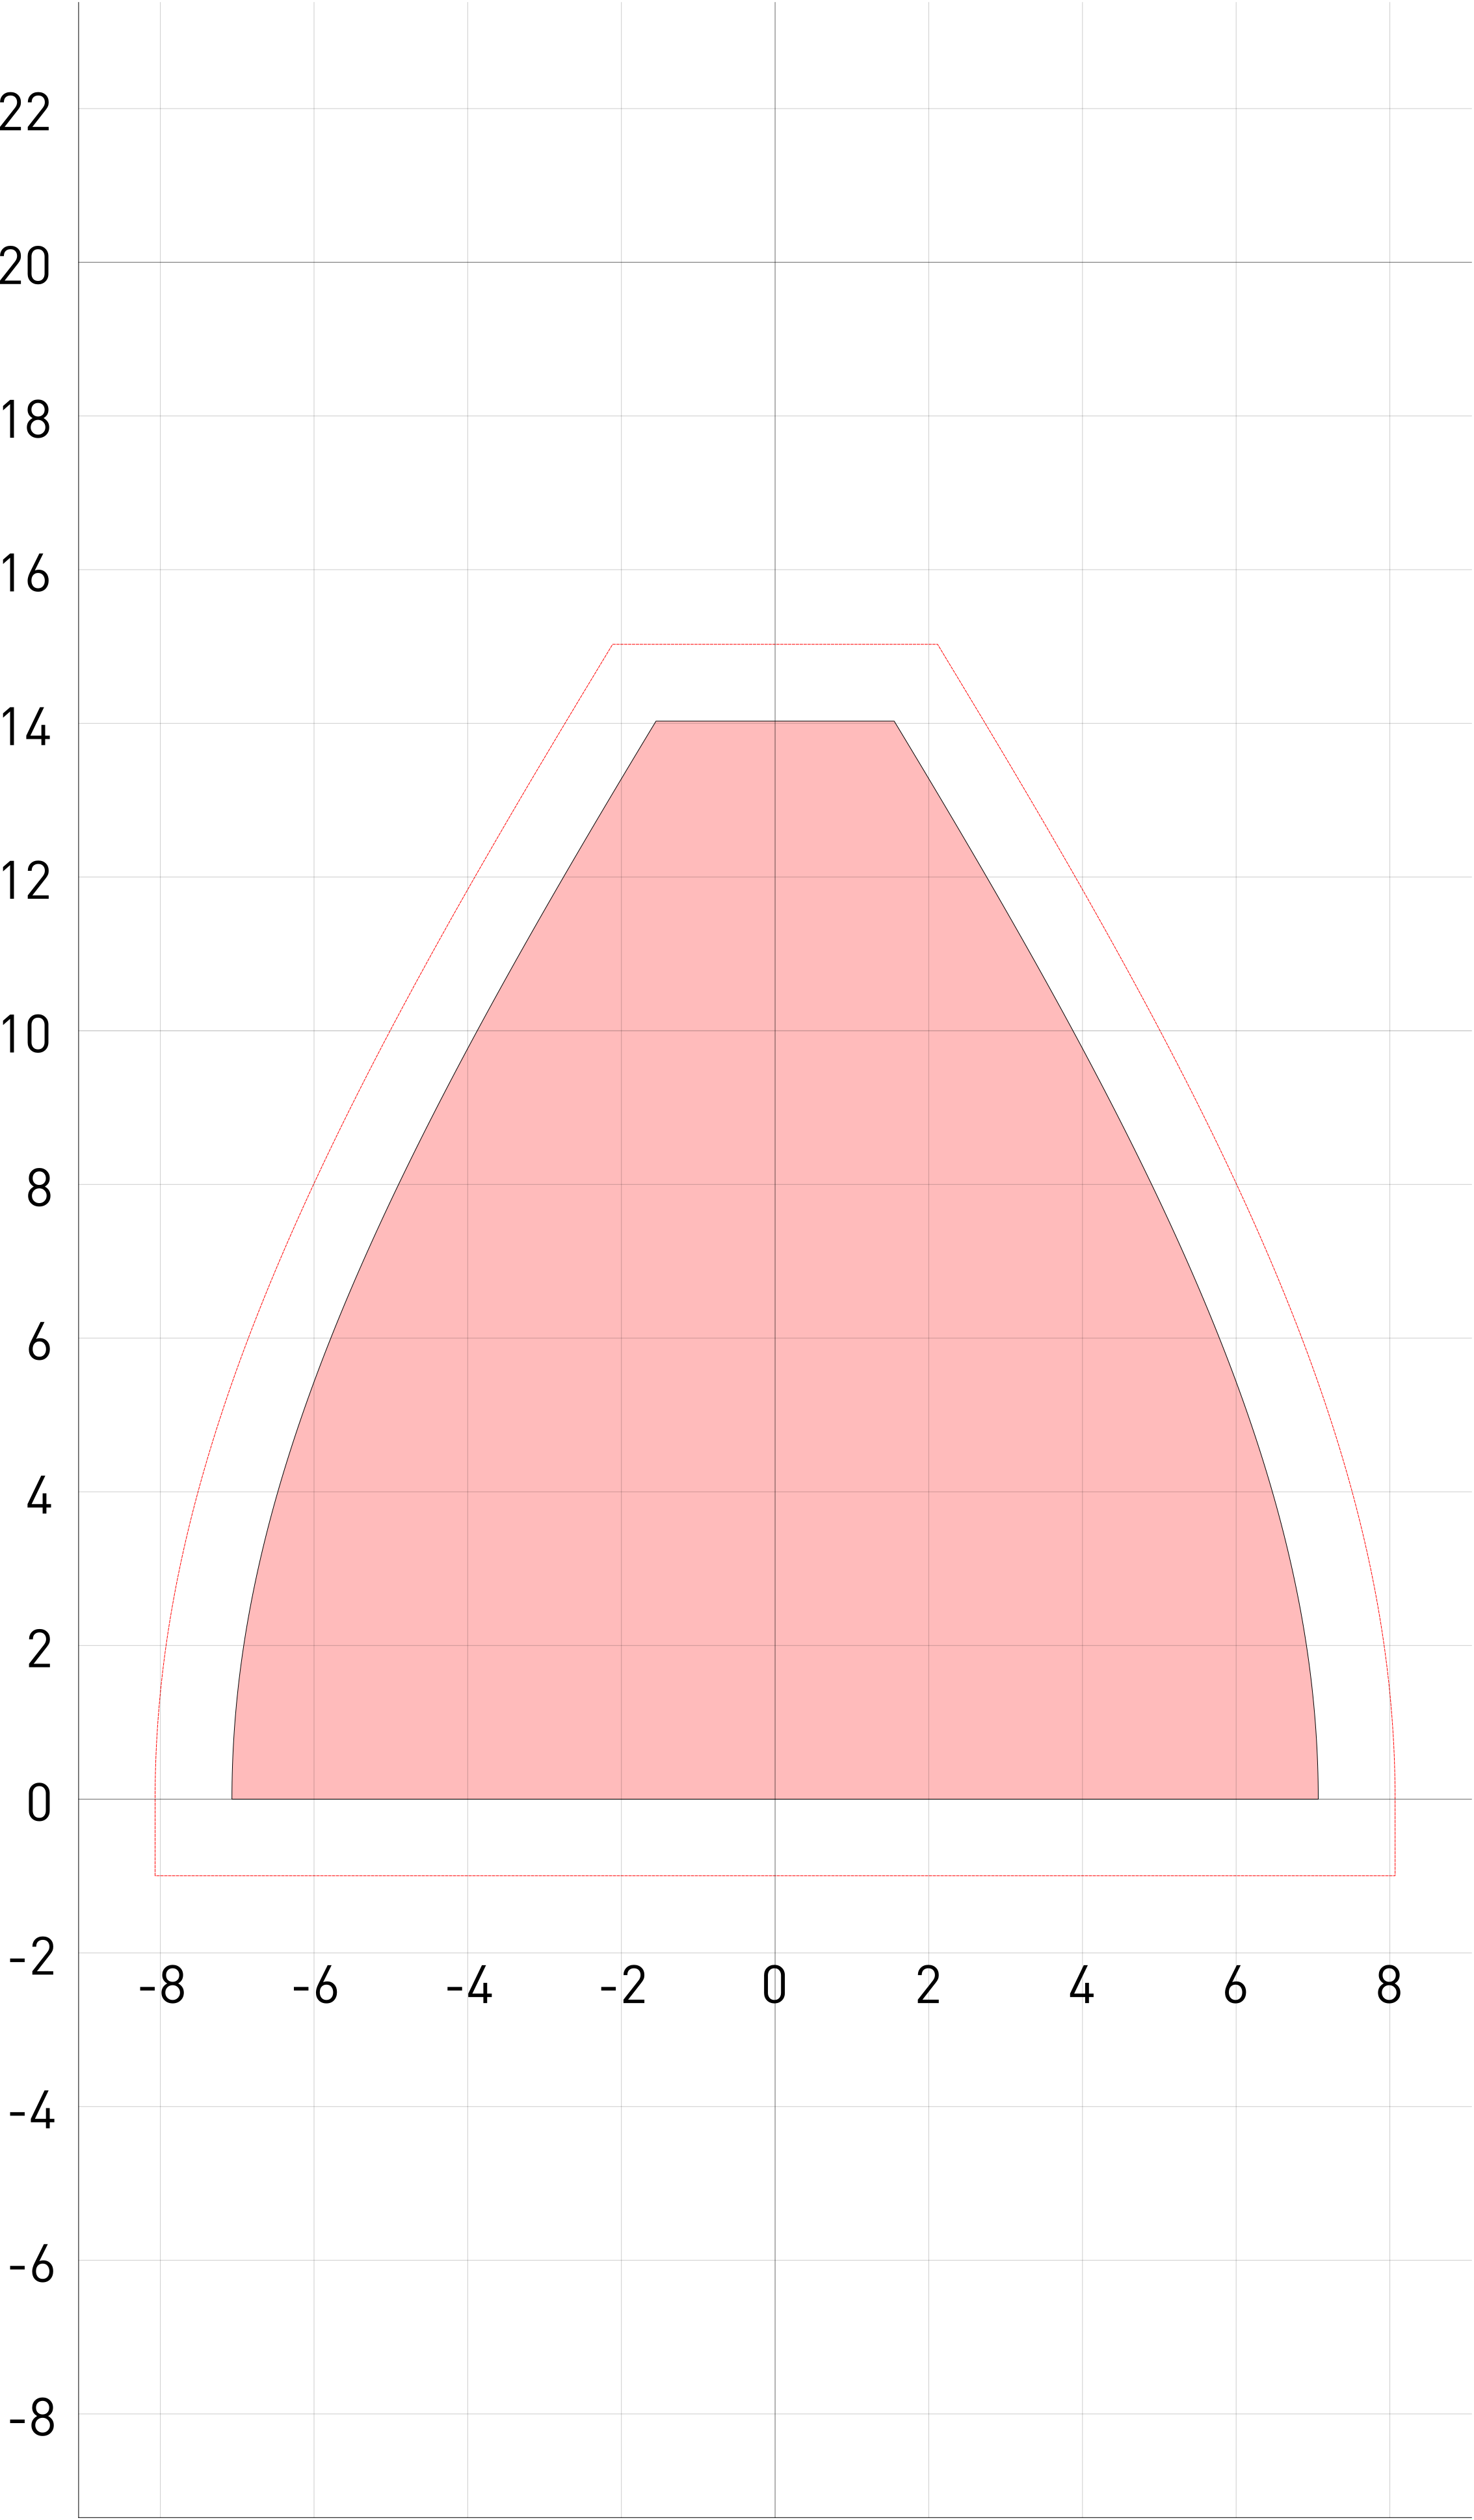
\includegraphics[width=5cm]{PlotItem_1.png}
    \end{minipage}
}